%-----------------------------------LICENSE------------------------------------%
%   This file is part of tikz_figures.                                         %
%                                                                              %
%   tikz_figures is free software: you can redistribute it and/or              %
%   modify it it under the terms of the GNU General Public License as          %
%   published by the Free Software Foundation, either version 3 of the         %
%   License, or (at your option) any later version.                            %
%                                                                              %
%   tikz_figures is distributed in the hope that it will be useful,            %
%   but WITHOUT ANY WARRANTY; without even the implied warranty of             %
%   MERCHANTABILITY or FITNESS FOR A PARTICULAR PURPOSE.  See the              %
%   GNU General Public License for more details.                               %
%                                                                              %
%   You should have received a copy of the GNU General Public License along    %
%   with tikz_figures.  If not, see <https://www.gnu.org/licenses/>.           %
%------------------------------------------------------------------------------%

% Use the standalone class for displaying the tikz image on a small PDF.
\documentclass[crop, tikz]{standalone}

% Import the tikz package to use for the drawing.
\usepackage{tikz}

% Tikz packages used.
\usetikzlibrary{arrows.meta, angles, quotes}

% Begin the document.
\begin{document}

    % Begin the drawing.
    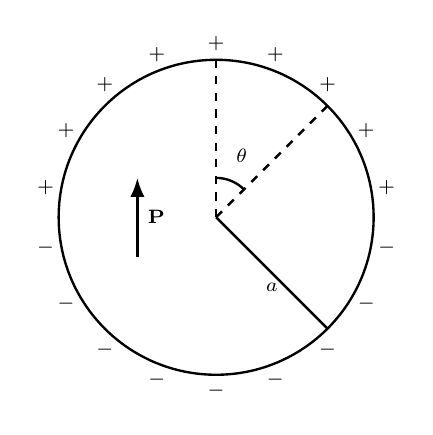
\begin{tikzpicture}[%
        font = \scriptsize,
        > = Latex,
        line width = 0.3mm
    ]

        % Positions for all of the points.
        \coordinate (O) at (0.0, 0.0);
        \coordinate (A) at (0.0, 2.0);
        \coordinate (B) at (1.414, 1.414);
        \coordinate (C) at (1.414, -1.414);
        \coordinate (D) at (-1.0, -0.5);
        \coordinate (E) at (-1.0, 0.5);

        % The circle the charges lie on and radial lines.
        \draw (O) circle (2);
        \draw[dashed] (O) to (A);
        \draw[dashed] (O) to (B);
        \draw (O) to node[below] {$a$} (C);

        % Arrow indicating direction of force.
        \draw[->] (D) to node[right] {$\mathbf{P}$} (E);

        % Draw and label the angle theta.
        \pic[%
            draw = black,
            "\scriptsize{${\theta}$}",
            angle eccentricity = 1.7,
            angle radius = 0.5cm
        ]   {angle = B--O--A};

        % Label all of the positive and negative charges on the circle.
        \foreach \a in {1, 3, ..., 17}{
            \draw (\a*360/36: 2.2) node{$+$};
            \draw (\a*360/36+180: 2.2) node{$-$};
        }
    \end{tikzpicture}
\end{document}
